\documentclass[11pt,oneside,a4paper,titlepage,onecolumn]{article}

\usepackage[utf8]{inputenc}
\usepackage{textcomp}
\usepackage[official]{eurosym}
\usepackage[polish]{babel}
\usepackage{amsthm}
\usepackage{graphicx}
\usepackage[T1]{fontenc}
\usepackage{scrextend}
\usepackage{hyperref}
\usepackage{xcolor}
% \usepackage{nameref}
% \usepackage{showlabels}
% \usepackage{titlesec}
\usepackage{geometry}
\geometry{a4paper, portrait, margin=2cm}
\graphicspath{ {./fig/} }

\newenvironment{enumreq}
{ \begin{enumerate}[topsep=0pt,itemsep=-1ex,partopsep=1ex,parsep=1ex] }
{ \end{enumerate}                  } 


\setcounter{secnumdepth}{4}

%% Author and title
\author{Marek Marecki \and Krzysztof Franek}
\title{%
    Proving viability of Viua VM \\
    \large Implementation of high-level language on Viua VM\\
    and deployment of simple application \\
    ~\\
    Projekt Systemu\\
    dla języka Viuact}

\begin{document}

\maketitle
{\footnotesize
\begin{center}
  \begin{tabular}{ | l | l | l | }
    \hline
    \parbox[t]{6.5cm}{\textbf{Temat pracy i akronim projektu:}\\Proving viablity of Viua VM (VVIA)} & \parbox[t]{4.5cm}{\textbf{Zleceniodawca:}\\\colorbox{yellow}{Nieznany}} & \parbox[t]{4.5cm}{\textbf{Konsultant:}\\\colorbox{yellow}{Nieznany}} \\ \hline
    \parbox[t]{6.5cm}{\textbf{Zespół projektowy:}\\Krzysztof Franek, Marek Marecki} & \parbox[t]{4.5cm}{\textbf{Kierownik projektu:}\\Marek Marecki} & \parbox[t]{4.5cm}{\textbf{Opiekun projektu:}\\dr hab. Marek A. Bednarczyk, prof. PJWSTK} \\ \hline
    \parbox[t]{3.5cm}{\textbf{Kierownik projektu:}\\Marek Marecki} &
      \multicolumn{2}{|l|}{\parbox[t]{9cm}{\textbf{Odpowiedzialny za dokument:}\\Marek Marecki}} \\ 
    \hline
  \end{tabular}
\end{center}
}

\tableofcontents
\newpage

\section{Architektura}

\subsection{Użyte wzorce projektowe -- Sposób konstrukcji kompilatora}

\begin{figure}[!htp]
    \centering
    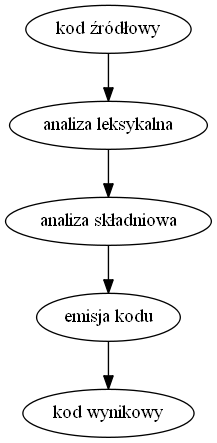
\includegraphics[width=5cm]{basic-compiler-flow}
    \caption{Podstawowy schemat budowy kompilatora}
    \label{basic_compiler_flow}
\end{figure}

Na rysunku \ref{basic_compiler_flow} przedstawiony jest uproszczony schemat budowy kompilatora.
W kompilatorach ''produkcyjnych'' (np. GCC, Clang, czy ICC) tych faz jest więcej -- przede wszystkim etap
emisji kodu jest dużo bardziej rozbudowany, oraz dochodzą etapy analizy semantycznej (czy program ma sens) czy
optymalizacji (prób takiego przekształcenia kodu programu żeby przy zachowaniu znaczenia działał wydajniej).

Kompilator języka ViuAct dostarczany jako element tej pracy inżynierskiej jest pozbawiony etapów
analizy semantycznej oraz optymalizacji. Analiza semantyczna (oraz weryfikacja typów i wykrywanie błędów na
etapie kompilacji) jest oddelegowana do assemblera dostarczanego przez platformę. Optymalizacja jest
całkowicie pominięta gdyż jest to temat niezwykle rozległy; implementacja i doszlifowanie algorytmów
optymalizujących kod jest sama w sobie materiałem wystarczającym na napisanie osobnej pracy inżynierskiej.

Architektura kompilatora języka ViuAct jest dokładniej opisana w rozdziale
\ref{architektura_kompilatora_viuact} (\nameref{architektura_kompilatora_viuact}) na
stronie \pageref{architektura_kompilatora_viuact}.
Sposób działania kompilatora jest opisany w rozdziale \ref{opis_etapow_kompilacji}
(\nameref{opis_etapow_kompilacji}) na stronie \pageref{opis_etapow_kompilacji}.
Omówienie interakcji kompilatora języka ViuAct z narzędziami dostarczanymi przez platformę Viua VM znajduje
się w rozdziale \ref{architektura_systemu} (\nameref{architektura_systemu}) na stronie
\pageref{architektura_systemu}.

\newpage

\subsection{Architektura systemu}
\label{architektura_systemu}

\begin{figure}[!htp]
    \centering
    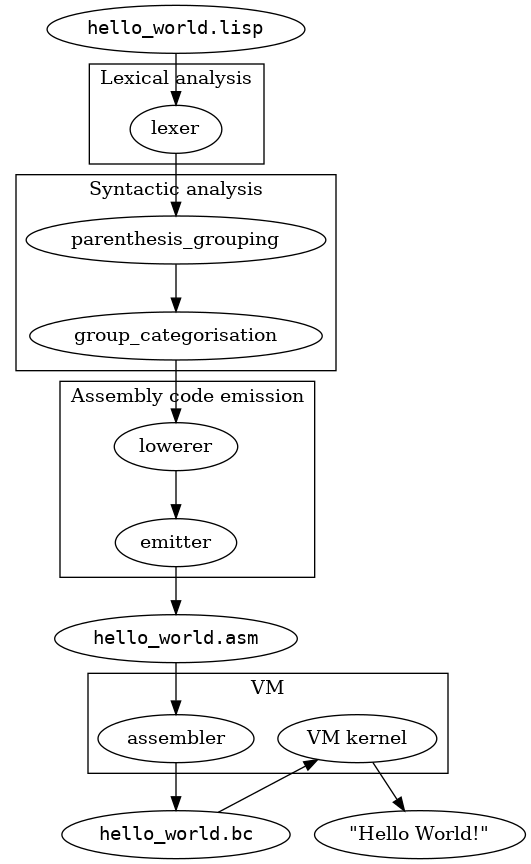
\includegraphics[width=10cm]{viuact-pipeline}
    \caption{Interakcje: od pliku źródłowego do działającego programu}
    \label{schemat_interakcji_viuact_z_viuavm}
\end{figure}

Rysunek \ref{schemat_interakcji_viuact_z_viuavm} (''\nameref{schemat_interakcji_viuact_z_viuavm}'') prezentuje
schemat interakcji jakie zachodzą w całym systemie od momentu wczytania pliku źródłowego przez kompilator do
uruchomienia programu przez jądro Viua VM.

Ostatnią fazą jaką zajmuje się kompilator języka ViuAct dostarczany jako element tej pracy inżynierskiej jest
emisja kodu (''Assembly code emission''), której wynikiem jest plik z kodem źródłowym w języku assemblera Viua
VM (''\texttt{hello\_world.asm}'' na rysunku). Rozdział \ref{architektura_kompilatora_viuact}
(\nameref{architektura_kompilatora_viuact}) dokładniej opisuje działanie samego kompilatora.

Zakres tej pracy inżynierskiej kończy się na wygenerowaniu pliku zawierającego poprawny kod w języku
assemblera Viua VM oraz plików pomocniczych (dokładniej opisanych w rozdziałach
''\nameref{pliki_interfejsow_modulow}'' na stronie \pageref{pliki_interfejsow_modulow} i
''\nameref{pliki_zaleznosci_modulow}'' na stronie \pageref{pliki_zaleznosci_modulow}).
Pliki pomocnicze są wymagane przez ''program łączący'' (opisany w rozdziale \ref{opis_linkera} na stronie
\pageref{opis_linkera}).

\subsection{Dekompozycja systemu na podsystemy}
\label{architektura_kompilatora_viuact}

\subsubsection{Kompilator -- \texttt{viuact-cc}}
\label{opis_kompilatora}

lexer -> parser -> lowerer -> emitter

\subsubsection{Program łączący -- \texttt{viuact-opt}}
\label{opis_linkera}

\subsection{Przepieg procesu kompilacji}
\label{opis_etapow_kompilacji}

Co po kolei robi kompilator.
Od wczytania pliku z kodem źródłowym do wyemitowania kodu wynikowego w języku assemblera.

\section{Projekt struktury}

\subsection{Diagram klas}

Brak diagramu klas, ponieważ jest zbędny (program nie jest pisany w stylu obiektowym).

\subsection{Opis zmian i uszczegółowień w stosunku do diagramu analitycznego}

\section{Wykorzystane elementy}

\emph{Wykorzystane komponenty, programy, itp.}

\section{Decyzje projektowe}

\subsection{Środowisko docelowe}

\subsection{Środowisko implementacji}

\subsection{Priorytety implementacyjne}

Maksymalizacja prostoty budowy kompilatora i języka.
Marginalizacja obsługi błędów w kompilatorze z uwagi na brak czasu.
Marginalizacja optymalizacji z uwagi na brak czasu.

\section{Projekt algorytmów i przyjętych protokołów}

\section{Projekt rozwiązań sprzętowych}

Brak w tym projekcie. Jest on wyłącznie softwareowy.

\section{Projekt interfejsu}

\subsection{Interfejs użytkownika}

\subsubsection{Założenia konstrukcji interfejsu}

\subsection{Interfejs kompilatora}

Kompilator składa się z dwóch programów: \texttt{viuact-cc} (kompilatora właściwego) i \texttt{viuact-opt}
(programu łączącego).

\subsection{Interfejs języka}

Interfejsem języka jest jego składnia.
Jest ona opisana w specyfikacji języka.

\subsection{Inne interfejsy}

\subsubsection{Pliki interfejsów modułów (\texttt{.i})}
\label{pliki_interfejsow_modulow}

\subsubsection{Pliki zależności modułów (\texttt{.d})}
\label{pliki_zaleznosci_modulow}

\section{Projekt bazy danych}

Brak bazy danych w projekcie.

\section{Opis implementacji}

Krótka dyskusja jak przyjęte rozwiązania projektowe spełniają wymagania, szczególnie jakościowe, np.
bezpieczeństwo.

\section{Załączniki}

Specyfikacja języka ViuAct -- ''\emph{viuact-specification.pdf}''.

\end{document}
